% assignment_6.tex - Assignment 6 for Data Fusion class (Fall 2014)
% Chanmann Lim - October 2014

\documentclass[a4paper]{article}

\usepackage[margin=1 in]{geometry}
\usepackage{amsmath}
\usepackage{listings}
\usepackage{graphicx}

\everymath{\displaystyle}

\begin{document}
\title{CS 8790: Solution to assignment 6}
\author{Chanmann Lim}
\date{October 27, 2014}
\maketitle

\subsection*{Report:} ~\\
\indent Suppose we have a rover deployed in a remote 2D environment and we would like to move the rover to a targeted position (in the 2D environment) by sending control input commanding the rover to move some distances relative to its current position. However various levels of uncertainties (in the remote environment or in some errors in the design of the rover) might affect the prediction of the location of the rover as it is traversing and to re-adjust our estimate we have the sensor that can observe the rover and provides independent and consistent (unbiased and conservative covariance) observation of its current position then we go through control input and observation loop until the rover reaches the desired location. \\
\\
\indent In maintaining the estimate of the state of the rover, the control inputs and the observations have to be treated differently. When the control input is sent the best estimate of the new location of the rover is just the sum of the rover's current position and the relative changes in position moreover the covariance of the two measurements also get added together. \\
\begin{align*}
x_{new} &= x + z \\
P_{new} &= P + R \\
\end{align*}
This reduces the value of information about our prediction and only until the new observation coming in can the estimate be fused using the Kalman filter to produce the new result which will lower the uncertainty introduced by prior control inputs. \\
\begin{align*}
P_{new} &= P - WSW^{T}\\
x_{new} &= x + W(z - Hx)\\
v &= S^{-\frac{1}{2}}(z-Hx)
\end{align*}
where
\begin{align*}
S &= HPH^{T} + R\\
W &= PH^{T}S^{-1}
\end{align*}

\paragraph{1. } The plot of the normalized innovations (for the observation that provides 2 innovations, the first is being chosen for plotting):\\
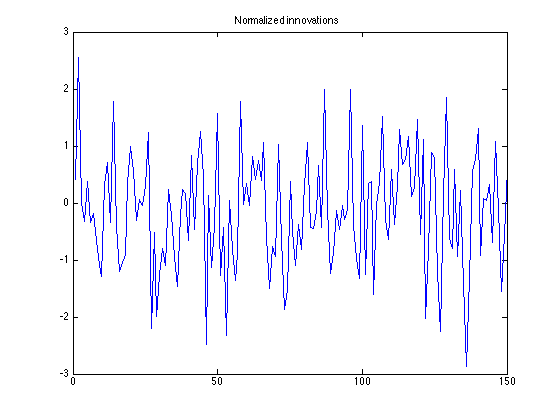
\includegraphics[scale=.70]{normalized_innovations.png}

\paragraph{2. } The square root of the trace of the rover covariance matrix is the distance from the rover estimated position and the true position calculated by taking the square root of sum of the diagonal values of its covariance matrix $P$
\begin{align*}
square\_root\_trace = \sqrt{sum(diag(P))}
\end{align*}\\
and the following is the plot of the square root of the trace of the rover covariance matrix for both when sending the control input and obtaining the observation : \\
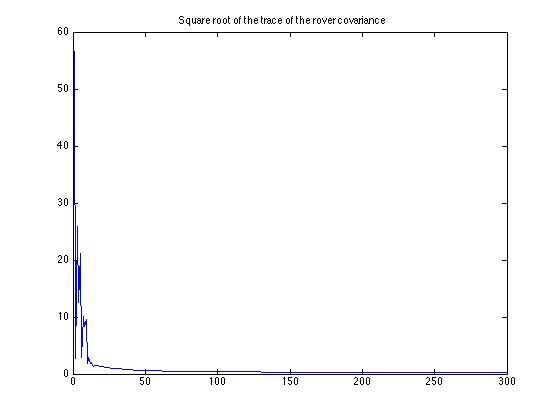
\includegraphics[scale=.7]{sqrt_traces.png}

\paragraph{3. } The rover's path position estimates after each control input: \\
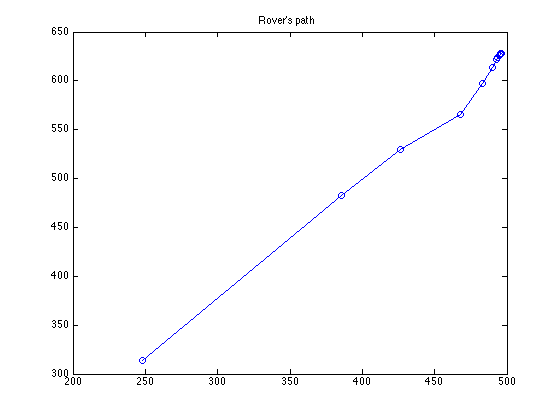
\includegraphics[scale=.75]{rover_path.png} \\
The rover moved a few fairly large distances at the beginning then started taking many granular steps to an exact target on the upper-right corner of the above plot and zooming in to the location will reveal the rover's maneuvers. \\
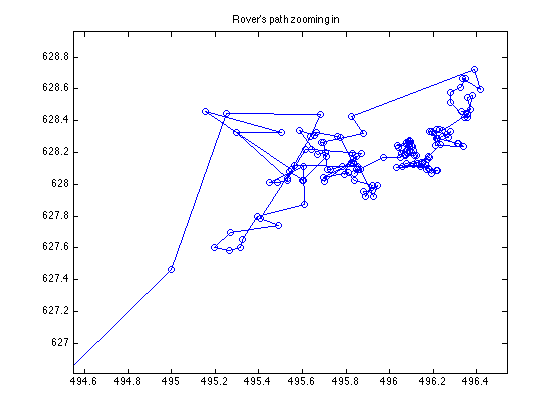
\includegraphics[scale=.75]{rover_path_zoom_in.png} \\

\paragraph{4. } The observations with innovation size less than 1 is 61.33\%.

\paragraph{5. } The rover's final estimated position is [495.868838, 628.111014] and the standard deviation can be obtained by taking the square root of diagonal elements of the covariance $P$ of the final position.\\
\begin{align*}
	x_{final} &=
	\begin{bmatrix}
		495.868838 \\
    	628.111014
	\end{bmatrix} \\
	standard\_deviation &=
	\begin{bmatrix}
		0.216657 \\
    	0.216158
	\end{bmatrix}
\end{align*}
\begin{align*}
	final\_estimate =
	\begin{pmatrix}
		495.868838 & 0.216657 \\
    	628.111014 & 0.216158
	\end{pmatrix}
\end{align*}

\newpage
\subsection*{Appendix:}
\lstinputlisting[language=Matlab, title=\lstname, basicstyle=\footnotesize]{assignment_6.m}
\lstinputlisting[language=Matlab, title=\lstname, basicstyle=\footnotesize]{get_observation.m}
\lstinputlisting[language=Matlab, title=\lstname, basicstyle=\footnotesize]{update.m}
\lstinputlisting[language=Matlab, title=\lstname, basicstyle=\footnotesize]{report.m}

\end{document}